\documentclass[]{tufte-handout}

% ams
\usepackage{amssymb,amsmath}

\usepackage{ifxetex,ifluatex}
\usepackage{fixltx2e} % provides \textsubscript
\ifnum 0\ifxetex 1\fi\ifluatex 1\fi=0 % if pdftex
  \usepackage[T1]{fontenc}
  \usepackage[utf8]{inputenc}
\else % if luatex or xelatex
  \makeatletter
  \@ifpackageloaded{fontspec}{}{\usepackage{fontspec}}
  \makeatother
  \defaultfontfeatures{Ligatures=TeX,Scale=MatchLowercase}
  \makeatletter
  \@ifpackageloaded{soul}{
     \renewcommand\allcapsspacing[1]{{\addfontfeature{LetterSpace=15}#1}}
     \renewcommand\smallcapsspacing[1]{{\addfontfeature{LetterSpace=10}#1}}
   }{}
  \makeatother

\fi

% graphix
\usepackage{graphicx}
\setkeys{Gin}{width=\linewidth,totalheight=\textheight,keepaspectratio}

% booktabs
\usepackage{booktabs}

% url
\usepackage{url}

% hyperref
\usepackage{hyperref}

% units.
\usepackage{units}


\setcounter{secnumdepth}{-1}

% citations
\usepackage{natbib}
\bibliographystyle{plainnat}

% pandoc syntax highlighting

% longtable

% multiplecol
\usepackage{multicol}

% strikeout
\usepackage[normalem]{ulem}

% morefloats
\usepackage{morefloats}


% tightlist macro required by pandoc >= 1.14
\providecommand{\tightlist}{%
  \setlength{\itemsep}{0pt}\setlength{\parskip}{0pt}}

% title / author / date
\title{Marketing Report}
\date{2020-11-13}

\usepackage{booktabs}
\usepackage{longtable}
\usepackage{array}
\usepackage{multirow}
\usepackage{wrapfig}
\usepackage{float}
\usepackage{colortbl}
\usepackage{pdflscape}
\usepackage{tabu}
\usepackage{threeparttable}
\usepackage{threeparttablex}
\usepackage[normalem]{ulem}
\usepackage{makecell}

\begin{document}

\maketitle




\hypertarget{description}{%
\section{Description}\label{description}}

\newthought{The purpose of this analysis} is to explore the changes that
have occurred in the flow of applications to Undergraduate Online
Programs. I look at both application data from past census reports and
inquiry data from prospective students who fill out Marketing inquiry
forms that can be filled out from campaign landing pages.

\hypertarget{findings}{%
\section{Findings}\label{findings}}

\newthought{FY20 saw an increase} in applications for students seeking
online programs. After a one year period that started in Aug, 2018,
marking a dearth of applications to the University's Undergraduate
Online Programs, applications started coming in at a higher rate. This
change is evident in the two plots below.

The first shows that there has been growth in the last census year.

\hypertarget{section}{%
\section{}\label{section}}

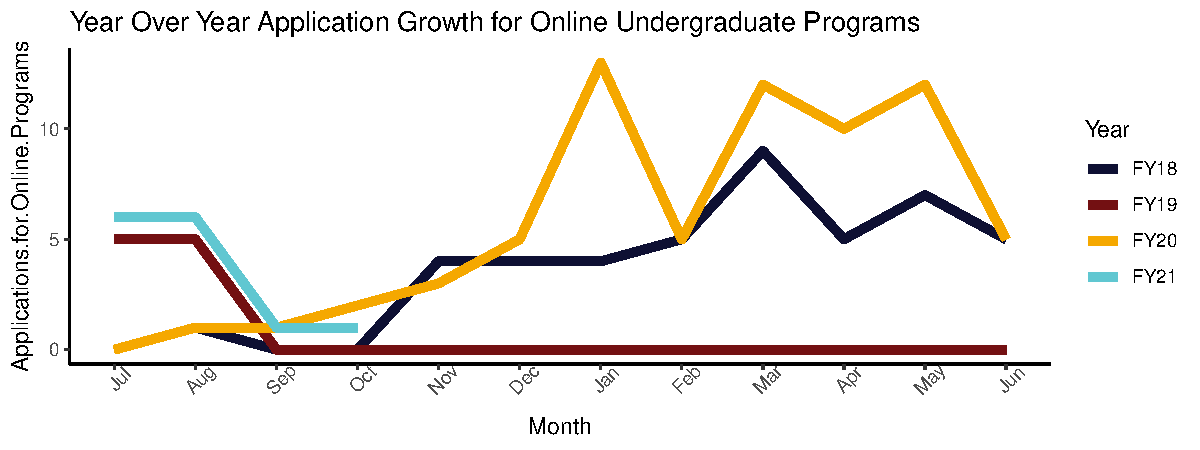
\includegraphics{FY20-Online-Application-Flow-as-of-Census-10-15-2020_files/figure-latex/unnamed-chunk-5-1}

The second plot, shown below, captures the same data on a time line. The
second period of activity, from August 2019, is significantly higher
that the previous period. This is very exciting.

\hypertarget{section-1}{%
\section{}\label{section-1}}

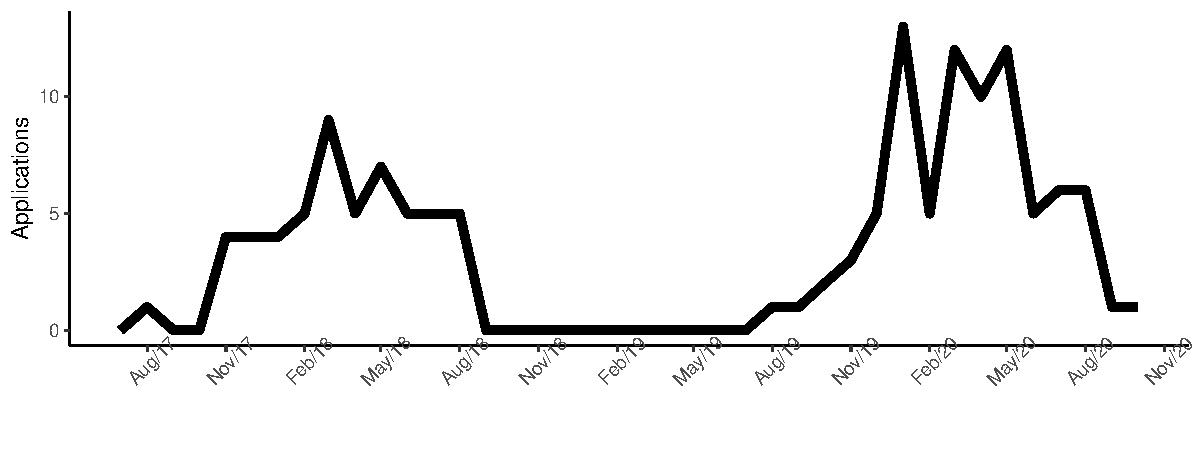
\includegraphics{FY20-Online-Application-Flow-as-of-Census-10-15-2020_files/figure-latex/unnamed-chunk-6-1}

The final plot, shown below, marks the flow of marketing inquiry forms
(as an initial referral source). What is clear is an increase in the
flow of inquiries preceded the growth in applications.

\hypertarget{section-2}{%
\section{}\label{section-2}}

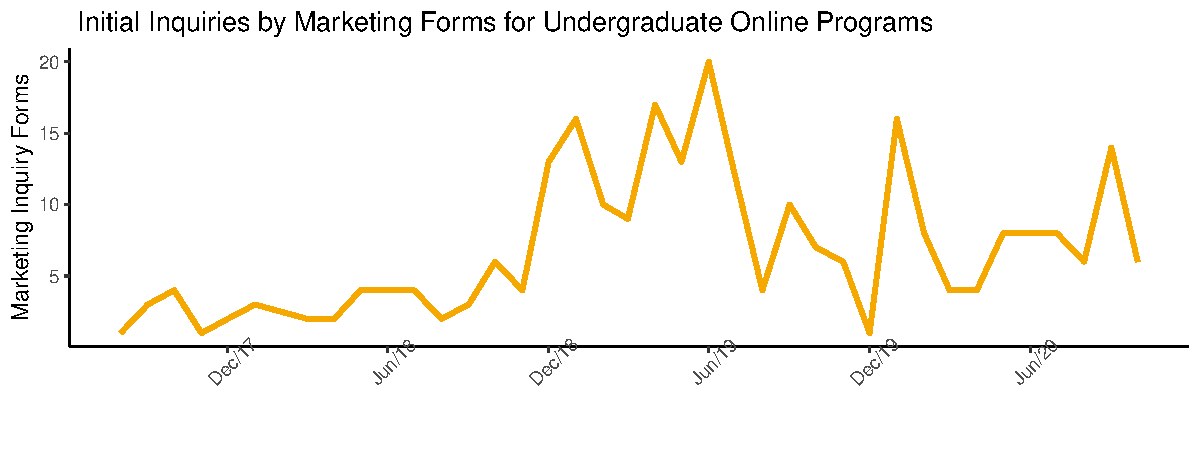
\includegraphics{FY20-Online-Application-Flow-as-of-Census-10-15-2020_files/figure-latex/unnamed-chunk-7-1}

\textbf{Age of Applicant}

\begin{table}[H]
\centering
\begin{tabular}{l|l|r}
\hline
FiscalYear & AgeGroup & Applications\\
\hline
FY20 & 19 and Under & 11\\
\hline
FY20 & 20-25 & 18\\
\hline
FY20 & 26 and Up & 39\\
\hline
FY21 & 20-25 & 2\\
\hline
FY21 & 26 and Up & 12\\
\hline
\end{tabular}
\end{table}

\hypertarget{conclusions}{%
\section{Conclusions}\label{conclusions}}

\begin{itemize}
\item
  While a small component of the University's portfolio of products,
  Online Programs have grown.
\item
  Further analysis into the the performance of ads for the online
  programs might show a similar trend.
\end{itemize}

\href{https://www.wrike.com/open.htm?id=589938175}{{\color{blue}{\underline{Wrike Project Details}}}}

\href{https://github.com/edithbird/online-programs-application-flow}{{\color{blue}{\underline{Github Repository}}}}

\begin{marginfigure}
Notice that there is no number preceding the note. \(x \in [a, b]\)有
\[\frac{d}{dx}\left( \int_{a}^{x} f(u)\,du\right)=f(x).\]
\end{marginfigure}

\bibliography{skeleton.bib}



\end{document}
